\documentclass[aspectratio=169,xcolor=table]{beamer}
\usetheme{metropolis}
\usepackage[spanish]{babel}
\usepackage{tikz}
\usetikzlibrary{chains}
\usetikzlibrary{trees}
\usepackage{minted}
\setminted{ style=colorful, fontsize=\small, breaklines}
\usepackage{xcolor-solarized}
\usepackage{fontawesome}
\usepackage{gitdags}

\newcommand{\twitter}{\href{https://twitter.com/carlosgllp}{\faTwitter\ carlosgllp}}
\newcommand{\github}{\href{https://www.github.com/gpcarlos}{\faGithub\ gpcarlos}}
\newcommand{\warnning}{{\color{solarized-red}\faWarning}}

\title{Taller de Git}
\subtitle{Avanzado}
\author{Carlos Gallardo Polanco \\ \twitter \\ \github}
\institute{Escuela Superior de Ingeniería}
\date{22 de mayo de 2018}
\subject{Actividad Científico-Técnica}
\keywords{ESI, UCA, Git, GitHub, LaTeX}

\definecolor{fafafa}{rgb}{0.98, 0.98, 0.98}
\newcommand{\whiteTitle}{
  \title{\color{fafafa}Taller de Git}
  \subtitle{\color{fafafa}Avanzado}
  \author{\color{fafafa}Carlos Gallardo Polanco \\ \twitter \\ \github}
  \institute{\color{fafafa}Escuela Superior de Ingeniería}
  \date{\color{fafafa}22 de mayo de 2018}
}

% ================================================
% ================================================
% ================================================

\begin{document}

\begin{frame}
  \maketitle
  \begin{tikzpicture}[remember picture,overlay]
    \node[anchor=north east,inner sep=40pt] at (current page.north east) {
\includegraphics[scale=0.065]{images/logoGit.png}};
    \node[anchor=south east,inner sep=40pt] at (current page.south east) {
\includegraphics[scale=0.3]{images/logoUCA.eps}};
  \end{tikzpicture}
\end{frame}

%  Conceptos básicos
\begin{frame}[fragile]{Comandos básicos - Iniciar un repositorio}
  \begin{columns}[onlytextwidth]
    \column{0.6\textwidth}
    \alert{Inicializar un repositorio}
    \begin{minted}{console}
    $ git init
    \end{minted}

    \alert{Clonar un repositorio de un remoto (\faGithubAlt GitHub!)}
    \begin{minted}{console}
    $ git clone <url>
    \end{minted}
    \column{0.4\textwidth}
    \tikzstyle{every node}=[draw=solarized-base1,thick,anchor=west]
    \tikzstyle{selected}=[draw=solarized-green,fill=solarized-green!30]
    \begin{tikzpicture}[%
      grow via three points={one child at (0.5,-0.7) and
      two children at (0.5,-0.7) and (0.5,-1.4)},
      edge from parent path={(\tikzparentnode.south) |- (\tikzchildnode.west)}]
      \node {directory}
        child { node [selected] {.git}}
        child { node {source}}
        child { node {LICENSE}}
        child { node {README.md}};
    \end{tikzpicture}
  \end{columns}
\end{frame}

\begin{frame}[fragile]{Comandos básicos - Preparar y confirmar}
  \alert{Añadir un archivo al área de preparación}
  \begin{minted}{console}
    $ git add <archivo>
  \end{minted}

  \alert{Confirmar los cambios}
  \begin{minted}{console}
    $ git commit
    $ git commit -m 'mensaje'
  \end{minted}

  \alert{Saltarse el área de preparación}
  \begin{minted}{console}
    $ git commit -a -m 'mensaje'
  \end{minted}
  \hspace{1cm} {\scriptsize Sólo prepara y confirma los archivos que Git está rastreando!}

  \begin{tikzpicture}[remember picture,overlay]
    \node[anchor=north east, inner xsep=45pt, inner ysep=60pt] at (current page.north east) {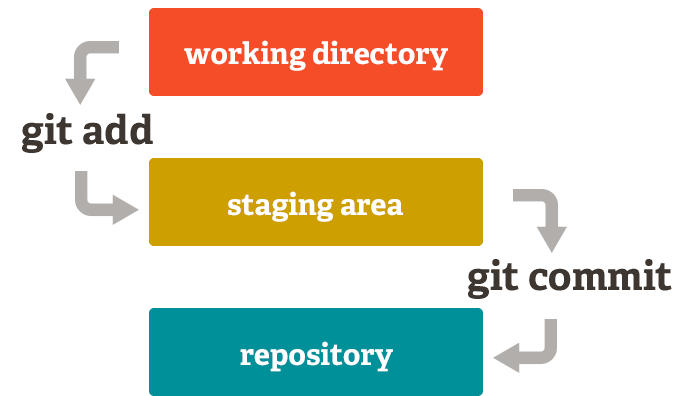
\includegraphics[scale=0.2]{images/areas}};
  \end{tikzpicture}
\end{frame}

\begin{frame}[fragile]{Comandos básicos - Revisar el estado}
  \begin{columns}[onlytextwidth]
  \column{0.35\textwidth}
  Diferencia entre archivos preparados, no preparados pero rastreados y no rastreados.
  \begin{minted}{console}
    $ git status
    $ git status -s
  \end{minted}
  \column{0.02\textwidth}
  \column{0.63\textwidth}
  \vspace{0.3cm}
  \begin{minted}[escapeinside=||, frame=single, framerule=1pt, fontsize=\scriptsize, bgcolor=solarized-base1!30]{console}
[user@linux ~]$ git status
On branch master
Changes to be committed:
(use "git reset HEAD <file>..." to unstage)
|  {\color{solarized-green}new file:   presentation.tex}|
|  {\color{solarized-green}deleted:    basura.text}|
Changes not staged for commit:
(use "git add <file>..." to update what will be committed)
(use "git checkout -- <file>..." to discard changes in working directory)
|  {\color{solarized-red}modified:   .gitignore}|
Untracked files:
(use "git add <file>..." to include in what will be committed)
|  {\color{solarized-red}configuration.tex}|
  \end{minted}
  \end{columns}
\end{frame}

% \begin{frame}[fragile]{Comandos básicos - Revisar el estado}
%   \begin{columns}[onlytextwidth]
%   \column{0.35\textwidth}
%   \begin{tabular}{rcl}
%     \texttt{A} & $\Rightarrow$ & Nuevo \\
%     \texttt{M} & $\Rightarrow$ & Modificado \\
%     \texttt{D} & $\Rightarrow$ & Eliminado \\
%     \texttt{?} & $\Rightarrow$ & No rastreado \\
%   \end{tabular}
%   \column{0.02\textwidth}
%   \column{0.63\textwidth}
%   \begin{minted}[escapeinside=||, frame=single, framerule=1pt, fontsize=\scriptsize, bgcolor=solarized-base1!30]{console}
% [user@linux ~]$ git status -s
% | {\color{solarized-red}M}| .gitignore
% |{\color{solarized-green}D} | basura.text
% |{\color{solarized-green}A} | presentation.tex
% |{\color{solarized-red}??}| configuration.tex
%   \end{minted}
%   \begin{center}
%   $1^a$ columna: En estado preparado \\
%   $2^a$ columna: En estado no preparado
%   \end{center}
%   \end{columns}
% \end{frame}

\begin{frame}[fragile]{Comandos básicos - Eliminar y Renombrar}
  \alert{Eliminar}
  \begin{itemize}
    \item Eliminar un archivo no preparado \warnning
    \begin{minted}{console}
  $ git rm <archivo>
    \end{minted}
    \item Eliminar un archivo preparado \warnning
    \begin{minted}{console}
  $ git rm -f <archivo>
    \end{minted}
    \item Eliminar del repositorio pero no del directorio de trabajo
    \begin{minted}{console}
  $ git rm --cached <archivo>
    \end{minted}
  \end{itemize}

  \alert{Renombrar}
  \begin{minted}{console}
    $ git mv <archivo> <archivo-nuevo>
  \end{minted}

\end{frame}


%  Ver el historial
\begin{frame}[fragile]{Ver el historial de confirmaciones}
  \begin{center}
  \begin{minted}{console}
                       $ git log <opciones>
  \end{minted}
  \alert{Opciones interesantes}
  \end{center}
  \begin{table}
  \rowcolors{1}{solarized-base01!20}{solarized-base01!15}
  \begin{tabular}{|r|l|} \hline
    \texttt{-p} & Diferencias \\ \hline
    \texttt{--stat} & Estadísticas \\ \hline
    \texttt{--shortstat} & Estadísticas resumidas \\ \hline
    \texttt{--name-only} & Lista de archivos afectados \\ \hline
    \texttt{--name-status} & Lista de archivos + estado \\ \hline
    \texttt{--abbrev-commit} & SHA-1 reducido \\ \hline
    \texttt{--relative-date} & Fecha en formato relativo \\ \hline
    \texttt{--graph} & Muestra un gráfico ASCII \\ \hline
    \texttt{--pretty=<op-pretty>} & Formato alternativo \\ \hline
  \end{tabular}
  \end{table}
\end{frame}

\begin{frame}[fragile]{Ver el historial de confirmaciones}
  \begin{center}
  \begin{minted}{console}
                   $ git log --pretty=<op-pretty>
  \end{minted}
  \alert{Opciones de format}
  \end{center}
  \begin{table}
  \rowcolors{1}{solarized-base01!20}{solarized-base01!15}
  \begin{tabular}{|r|l|} \hline
    \texttt{oneline} & SHA-1 y mensaje \\ \hline
    \texttt{short} & SHA-1, mensaje y autor \\ \hline
    \texttt{full} & SHA-1, mensaje, autor y confirmadores \\ \hline
    \texttt{fuller} & SHA-1, mensaje, autor, confirmadores y fechas \\ \hline
    \texttt{format} & Formato personalizado (\href{https://git-scm.com/docs/pretty-formats}{info}) \\ \hline
  \end{tabular}
  \end{table}
\end{frame}

\begin{frame}[fragile]{Ver el historial de confirmaciones}
  \begin{center}
  \begin{minted}{console}
                       $ git log <opciones>
  \end{minted}
  \alert{Opciones para limitar la salida}
  \end{center}
  \begin{table}
  \rowcolors{1}{solarized-base01!20}{solarized-base01!15}
  \begin{tabular}{|r|p{6cm}|} \hline
    \texttt{-<n>} & \texttt{n} últimas confirmaciones \\ \hline
    \texttt{--since=<f>}, \texttt{--after=<f>} & Confirmaciones despues la fecha \texttt{f}\\ \hline
    \texttt{--until=<f>}, \texttt{--before=<f>} & Confirmaciones hasta la fecha \texttt{f} \\ \hline
    \texttt{--author=<c>}, \texttt{--committer=<c>} & Confirmaciones del ser \texttt{c} \\ \hline
    \texttt{--merges}, \texttt{--no-merges} & Merges o no merges \\ \hline
    \texttt{--grep <cadena>} & \texttt{cadena} está en el mensaje \\ \hline
    \texttt{-S<cadena>} & Modifican código coincidente \newline con \texttt{cadena} \\ \hline
  \end{tabular}
  \end{table}
\end{frame}


%  Comprobar cambio
\begin{frame}[fragile]{Ver los cambios Preparados y No Preparados}
  Ver los cambios de un archivo respecto a su última confirmación
  \begin{itemize}
    \item \alert{Archivo no preparado}
    \begin{minted}{console}
      $ git diff <archivo>
    \end{minted}
    \item \alert{Archivo preparado}
    \begin{minted}{console}
      $ git diff --cached <archivo>
    \end{minted}
  \end{itemize}
\end{frame}


%  Volver atrás en el historial
\begin{frame}{Deshacer cosas}
  \begin{columns}[onlytextwidth]
    \column{0.7\textwidth}
    \begin{itemize}
      \item \alert{Rehacer el último commit}
        \mint{console}| $ git commit --amend|
      \item \alert{Deshacer un archivo preparado}
        \mint{console}| $ git reset HEAD <archivo>|
      \item \alert{Deshacer los cambios de todos los archivos} \warnning
        \mint{console}| $ git reset --hard HEAD|
      \item \alert{Deshacer los cambios un archivo modificado} \warnning
        \mint{console}| $ git checkout -- <archivo>|
        {\scriptsize \hspace{0.5cm} Sólo para archivos no preparados}
    \end{itemize}
    \column{0.3\textwidth}
      
\includegraphics[scale=0.2]{images/marty-mcfly}
  \end{columns}
\end{frame}

\begin{frame}{Deshacer cosas}
  \begin{columns}[onlytextwidth]
    \column{0.7\textwidth}
    \begin{itemize}
      \item \alert{Deshacer el último commit} \warnning
        \mint{console}| $ git reset HEAD~1|
      \item \alert{Deshacer los \texttt{n} últimos commits} \warnning
        \mint{console}| $ git reset HEAD~<n>|
      \item \alert{Deshacer commits desechando los cambios en el área de trabajo} \warnning
        \mint{console}| $ git checkout --hard HEAD~<n>|
    \end{itemize}
    \column{0.3\textwidth}
      
\includegraphics[scale=0.2]{images/marty-mcfly}
  \end{columns}
\end{frame}


%  Crear ramas y moverse entre ramas
\begin{frame}[fragile]{Ramificación}
    \begin{columns}[T,onlytextwidth]
      \column{0.55\textwidth}
      \begin{itemize}
        \item \alert{Crear una rama}
          \mint{console}| $ git branch <nombre-rama>|
        \item \alert{Moverse entre ramas}
          \mint{console}| $ git checkout <nombre-rama>|
        \item \alert{Crear y moverse a la rama creada}
          \mint{console}| $ git checkout -b <nombre-rama>|
      \end{itemize}
      \column{0.45\textwidth}
        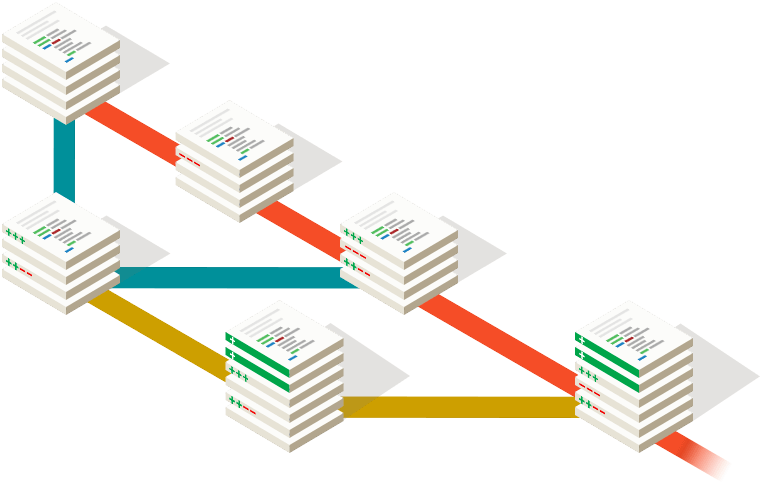
\includegraphics[scale=0.23]{images/branching-illustration}
    \end{columns}
\end{frame}

\begin{frame}[fragile]{Ramificación}
    \begin{columns}[T,onlytextwidth]
      \column{0.52\textwidth}
      \begin{exampleblock}{Ejemplo:}
        \uncover<2->{
        \mint{console}| $ git checkout -b issue53|}
        \uncover<3->{
        \mint{console}| $ git commit -am 'mensaje'|}
        \uncover<4->{
        \mint{console}| $ git checkout master|}
        \uncover<5->{
        \mint{console}| $ git checkout -b hotfix|}
        \uncover<6->{
        \mint{console}| $ git commit -am 'mensaje'|}
      \end{exampleblock}
      \column{0.48\textwidth}
        \begin{figure}
          \only<1>{\scalebox{.95}{\begin{tikzpicture}
  \gitDAG[grow right sep = 1.5em]{
    A -- B -- C
  };
  \gitbranch
    {master}      % node name and text
    {above=of C} % node placement
    {C}          % target
  % HDAD reference
  \gitHEAD
    {above=of master} % node placement
    {master}          % target
\end{tikzpicture}
}}
          \only<2>{\scalebox{.95}{\begin{tikzpicture}
  \gitDAG[grow right sep = 1.5em]{
    A -- B -- C
  };
  \gitbranch
    {master}      % node name and text
    {above=of C} % node placement
    {C}          % target
  \gitbranch
    {issue53}      % node name and text
    {below=of C} % node placement
    {C}          % target
  % HDAD reference
  \gitHEAD
    {below=of issue53} % node placement
    {issue53}          % target
\end{tikzpicture}
}}
          \only<3>{\scalebox{.95}{\begin{tikzpicture}
  \gitDAG[grow right sep = 1.5em]{
    A -- B -- C -- D
  };
  \gitbranch
    {master}      % node name and text
    {above=of C} % node placement
    {C}          % target
  \gitbranch
    {issue53}      % node name and text
    {below=of D} % node placement
    {D}          % target
  % HDAD reference
  \gitHEAD
    {below=of issue53} % node placement
    {issue53}          % target
\end{tikzpicture}
}}
          \only<4>{\scalebox{.95}{\begin{tikzpicture}
  \gitDAG[grow right sep = 1.5em]{
    A -- B -- C -- E
  };
  \gitbranch
    {master}      % node name and text
    {above=of C} % node placement
    {C}          % target
  \gitbranch
    {hotfix}      % node name and text
    {below=of E} % node placement
    {E}          % target
  % HDAD reference
  \gitHEAD
    {above=of master} % node placement
    {master}          % target
\end{tikzpicture}
}}
          \only<5>{\scalebox{.95}{\begin{tikzpicture}
  \gitDAG[grow right sep = 1.5em]{
    A -- B -- C -- {
    E,
    D},
  };
  \gitbranch
    {master}      % node name and text
    {above=of E} % node placement
    {E}          % target
  \gitbranch
    {issue53}      % node name and text
    {below=of D} % node placement
    {D}          % target
  % HDAD reference
  \gitHEAD
    {above=of master} % node placement
    {master}          % target
\end{tikzpicture}
}}
          \only<6>{\scalebox{.95}{\begin{tikzpicture}
  \gitDAG[grow right sep = 1.5em]{
    A -- B -- C -- {
    E,
    D},
  };
  \gitbranch
    {master}      % node name and text
    {above=of C} % node placement
    {C}          % target
  \gitbranch
    {issue53}      % node name and text
    {below=of D} % node placement
    {D}          % target
  \gitbranch
    {hotfix}      % node name and text
    {above=of E} % node placement
    {E}          % target
  % HDAD reference
  \gitHEAD
    {above=of hotfix} % node placement
    {hotfix}          % target
\end{tikzpicture}
}}
        \end{figure}
    \end{columns}
\end{frame}


%  Fusionar ramas
\begin{frame}[fragile]{Fusión de ramas}
    \begin{columns}
      \column{0.48\textwidth}
        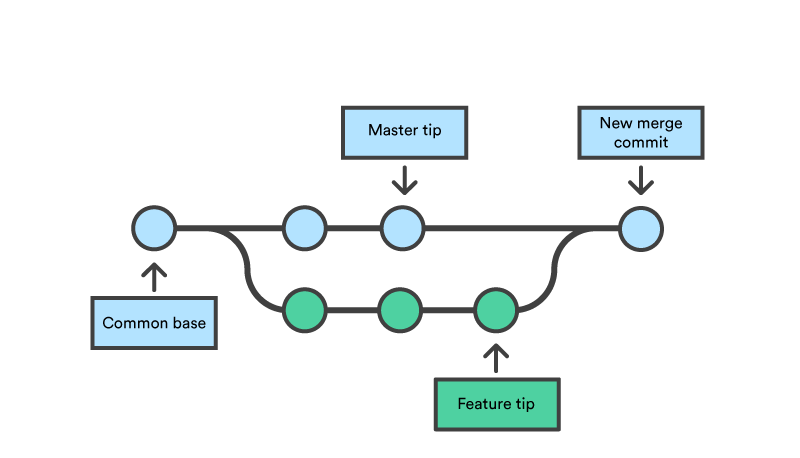
\includegraphics[scale=0.27]{images/branch-bitbucket}
      \column{0.52\textwidth}
      Si queremos fusionar dos ramas, nos posicionamos en la rama donde queremos que se apliquen los cambios y ejecutamos:
      \mint{console}| $ git merge <rama-a-fusionar>|
    \end{columns}
\end{frame}

\begin{frame}[fragile]{Fusión de ramas - \textsc{Fast-Forward}}
    \begin{columns}[onlytextwidth]
      \column{0.52\textwidth}
      \begin{exampleblock}{Ejemplo \textsc{Fast-Forward}:}
        \uncover<2->{
        \mint{console}| $ git checkout master|}
        \uncover<3->{
        \mint{console}| $ git merge hotfix|
        {\scriptsize \hspace{0.5cm} Adelanta el puntero de \texttt{master} a \texttt{hotfix}}}
        \uncover<4->{
        \mint{console}| $ git branch -d hotfix|}
      \end{exampleblock}
      \column{0.48\textwidth}
        \begin{figure}
          \only<1>{\scalebox{.95}{ \begin{tikzpicture}
  \gitDAG[grow right sep = 1.5em]{
    A -- B -- C -- {
    E,
    D},
  };
  \gitbranch
    {master}      % node name and text
    {above=of C} % node placement
    {C}          % target
  \gitbranch
    {issue53}      % node name and text
    {below=of D} % node placement
    {D}          % target
  \gitbranch
    {hotfix}      % node name and text
    {above=of E} % node placement
    {E}          % target
  % HDAD reference
  \gitHEAD
    {above=of hotfix} % node placement
    {hotfix}          % target
\end{tikzpicture}
}}
          \only<2>{\scalebox{.95}{ \begin{tikzpicture}
  \gitDAG[grow right sep = 1.5em]{
    A -- B -- C -- {
    E,
    D},
  };
  \gitbranch
    {master}      % node name and text
    {above=of C} % node placement
    {C}          % target
  \gitbranch
    {issue53}      % node name and text
    {below=of D} % node placement
    {D}          % target
  \gitbranch
    {hotfix}      % node name and text
    {above=of E} % node placement
    {E}          % target
  % HEAD reference
  \gitHEAD
    {above=of master} % node placement
    {master}          % target
\end{tikzpicture}
}}
          \only<3>{\scalebox{.95}{ \begin{tikzpicture}
  \gitDAG[grow right sep = 1.5em]{
    A -- B -- C -- {
    E,
    D},
  };
  \gitbranch
    {master}      % node name and text
    {above=of hotfix} % node placement
    {hotfix}          % target
  \gitbranch
    {issue53}      % node name and text
    {below=of D} % node placement
    {D}          % target
  \gitbranch
    {hotfix}      % node name and text
    {above=of E} % node placement
    {E}          % target
  % HEAD reference
  \gitHEAD
    {left=of master} % node placement
    {master}          % target
\end{tikzpicture}
}}
          \only<4>{\scalebox{.95}{ \begin{tikzpicture}
  \gitDAG[grow right sep = 1.5em]{
    A -- B -- C -- {
    E,
    D},
  };
  \gitbranch
    {master}      % node name and text
    {above=of E} % node placement
    {E}          % target
  \gitbranch
    {issue53}      % node name and text
    {below=of D} % node placement
    {D}          % target
  % HEAD reference
  \gitHEAD
    {above=of master} % node placement
    {master}          % target
\end{tikzpicture}
}}
        \end{figure}
    \end{columns}
\end{frame}

\begin{frame}[fragile]{Fusión de ramas - \textsc{3-way}}
    \begin{columns}[onlytextwidth]
      \column{0.52\textwidth}
      \begin{exampleblock}{Ejemplo \textsc{3-way}:}
        \uncover<2->{
        \mint{console}| $ git checkout master|}
        \uncover<3->{
        \mint{console}| $ git merge issue53|
        {\scriptsize \hspace{0.5cm} Crea un nuevo commit con la fusión a tres bandas de \\ \hspace{0.5cm} \texttt{master}, \texttt{issue53} y el \textbf{ancestro común} a ambas.}}
        \uncover<4->{
        \mint{console}| $ git branch -d issue53|}
      \end{exampleblock}
      \column{0.48\textwidth}
        \begin{figure}
          \only<1>{\scalebox{.85}{ \begin{tikzpicture}
  \gitDAG[grow right sep = 1.5em]{
    A -- B -- C -- {
    E -- G,
    D -- F},
  };
  \gitbranch
    {master}      % node name and text
    {above=of G} % node placement
    {G}          % target
  \gitbranch
    {issue53}      % node name and text
    {below=of F} % node placement
    {F}          % target
  % HEAD reference
  \gitHEAD
    {below=of issue53} % node placement
    {issue53}          % target
\end{tikzpicture}
}}
          \only<2>{\scalebox{.85}{ \begin{tikzpicture}
  \gitDAG[grow right sep = 1.5em]{
    A -- B -- C -- {
    E -- G,
    D -- F},
  };
  \gitbranch
    {master}      % node name and text
    {above=of G} % node placement
    {G}          % target
  \gitbranch
    {issue53}      % node name and text
    {below=of F} % node placement
    {F}          % target
  % HEAD reference
  \gitHEAD
    {above=of master} % node placement
    {master}          % target
\end{tikzpicture}
}}
          \only<3>{\scalebox{.80}{ \begin{tikzpicture}
  \gitDAG[grow right sep = 1.5em]{
    A -- B -- {[nodes=highlighted commit] {C}} -- {
      E -- {[nodes=highlighted commit] {G}} -- H,
      D -- {[nodes=highlighted commit] {F}} -- H},
  };
  \gitbranch
    {master}      % node name and text
    {above=of H} % node placement
    {H}          % target
  \gitbranch
    {issue53}      % node name and text
    {below=of F} % node placement
    {F}          % target
  % HEAD reference
  \gitHEAD
    {above=of master} % node placement
    {master}          % target
\end{tikzpicture}
}}
          \only<4>{\scalebox{.80}{ \begin{tikzpicture}
  \gitDAG[grow right sep = 1.5em]{
    A -- B -- C -- {
    E -- G -- H,
    D -- F -- H},
  };
  \gitbranch
    {master}      % node name and text
    {above=of H} % node placement
    {H}          % target
  % HEAD reference
  \gitHEAD
    {above=of master} % node placement
    {master}          % target
\end{tikzpicture}
} \\ \vspace{1.45cm}}
        \end{figure}
    \end{columns}
\end{frame}


%  Gestionar ramas
\begin{frame}{Gestionar ramas}
  \begin{itemize}
    \item \alert{Ver ramas}
      \mint{console}| $ git branch -v|
      {\scriptsize \ \ \texttt{-v}: Ver última confirmación de la rama} \\
      {\scriptsize \ \ \texttt{*}: Rama a la que apunta HEAD}
    \item \alert{Ver ramas que fusionadas con la rama activa}
      \mint{console}| $ git branch --merged|
      {\scriptsize \ \ Las ramas no activas pueden eliminarse ya que su contenido se ha incorporado a otras ramas} \\
      {\scriptsize \ \ \texttt{--no-merged}: Ramas no fusionadas con la rama activa}
    \item \alert{Eliminar ramas}
      \mint{console}| $ git branch -d <nombre-rama>|
  \end{itemize}
\end{frame}


%  Reorganizar ramas
\begin{frame}[fragile]{Reorganización de ramas}
  Podemos coger los cambios confirmados de una ramas \\ y reaplicarlos en otra.
  \mint{console}| $ git rebase <rama-en-la-cual-reorganizar>|
  \warnning {\color{solarized-red} \ La reorganización altera el historial}
\end{frame}

\begin{frame}[fragile]{Reorganización de ramas }
    \begin{columns}[onlytextwidth]
      \column{0.52\textwidth}
      \begin{exampleblock}{Ejemplo:}
        \uncover<2->{
        \mint{console}| $ git rebase master|}
        \uncover<3->{
        \mint{console}| $ git checkout master|}
        \uncover<4->{
        \mint{console}| $ git merge experiment|
        {\scriptsize \hspace{0.5cm} \texttt{Fast-Forward}}}
      \end{exampleblock}
      \column{0.48\textwidth}
        \begin{figure}
          \only<1>{\scalebox{.95}{ \begin{tikzpicture}
  \gitDAG[grow right sep = 1.5em]{
    A -- B -- C -- {
    E,
    D},
  };
  \gitbranch
    {master}      % node name and text
    {above=of E} % node placement
    {E}          % target
  \gitbranch
    {experiment}      % node name and text
    {below=of D} % node placement
    {D}          % target
  % HEAD reference
  \gitHEAD
    {below=of experiment} % node placement
    {experiment}          % target
\end{tikzpicture}
}}
          \only<2>{\scalebox{.95}{ \begin{tikzpicture}
  \gitDAG[grow right sep = 1.5em]{
    A -- B -- C -- {
    E -- D',
    {[nodes=unreachable] {D}}},
  };
  \gitbranch
    {master}      % node name and text
    {above=of E} % node placement
    {E}          % target
  \gitbranch
    {experiment}      % node name and text
    {above=of D'} % node placement
    {D'}          % target
  % HEAD reference
  \gitHEAD
    {above=of experiment} % node placement
    {experiment}          % target
\end{tikzpicture}
}}
          \only<3>{\scalebox{.95}{ \begin{tikzpicture}
  \gitDAG[grow right sep = 1.5em]{
    A -- B -- C -- {
    E -- D',
    {[nodes=unreachable] {D}}},
  };
  \gitbranch
    {master}      % node name and text
    {above=of E} % node placement
    {E}          % target
  \gitbranch
    {experiment}      % node name and text
    {above=of D'} % node placement
    {D'}          % target
  % HEAD reference
  \gitHEAD
    {above=of master} % node placement
    {master}          % target
\end{tikzpicture}
}}
          \only<4>{\scalebox{.95}{ \begin{tikzpicture}
  \gitDAG[grow right sep = 1.5em]{
    A -- B -- C -- {
    E -- D',
    {[nodes=unreachable] {D}}},
  };
  \gitbranch
    {master}      % node name and text
    {above=of D'} % node placement
    {D'}          % target
  \gitbranch
    {experiment}      % node name and text
    {below=of D'} % node placement
    {D'}          % target
  % HEAD reference
  \gitHEAD
    {above=of master} % node placement
    {master}          % target
\end{tikzpicture}
}}
        \end{figure}
    \end{columns}
\end{frame}


%  Remotos (pull y push)
\begin{frame}{Trabajar con Remotos}
  \begin{itemize}
    \item \alert{Ver tus remotos}
      \mint{console}| $ git remote -v|
    \item \alert{Añadir un remoto}
      \mint{console}| $ git remote add <nombre-remoto> <url>|
    \item \alert{Inspeccionar un remoto}
      \mint{console}| $ git remote show <nombre-remoto>|
    \item \alert{Eliminar un remoto}
      \mint{console}| $ git remote rm <nombre-remoto>|
    \item \alert{Renombrar un remoto}
      \mint{console}| $ git remote rename <nombre> <nombre-nuevo>|
  \end{itemize}
\end{frame}

\begin{frame}{Trabajar con Remotos}
  \begin{itemize}
    \item \alert{Traer remotos}
      \mint{console}| $ git fetch <nombre-remoto>|
      {\scriptsize Creará una nueva rama con el trabajo del remoto}
    \item \alert{Traer y Combinar remotos}
      \mint{console}| $ git pull <nombre-remoto> <nombre-rama>|
      \texttt{push = fetch + merge}
    \item \alert{Enviar a tus remotos}
      \mint{console}| $ git push <nombre-remoto> <nombre-rama>|
  \end{itemize}
  Si nuestra rama sigue a la rama remota, se puede no especificar nombres
  \begin{tikzpicture}[remember picture,overlay]
    \node[anchor=north east,inner ysep=50pt, inner xsep=20pt] at (current page.north east) {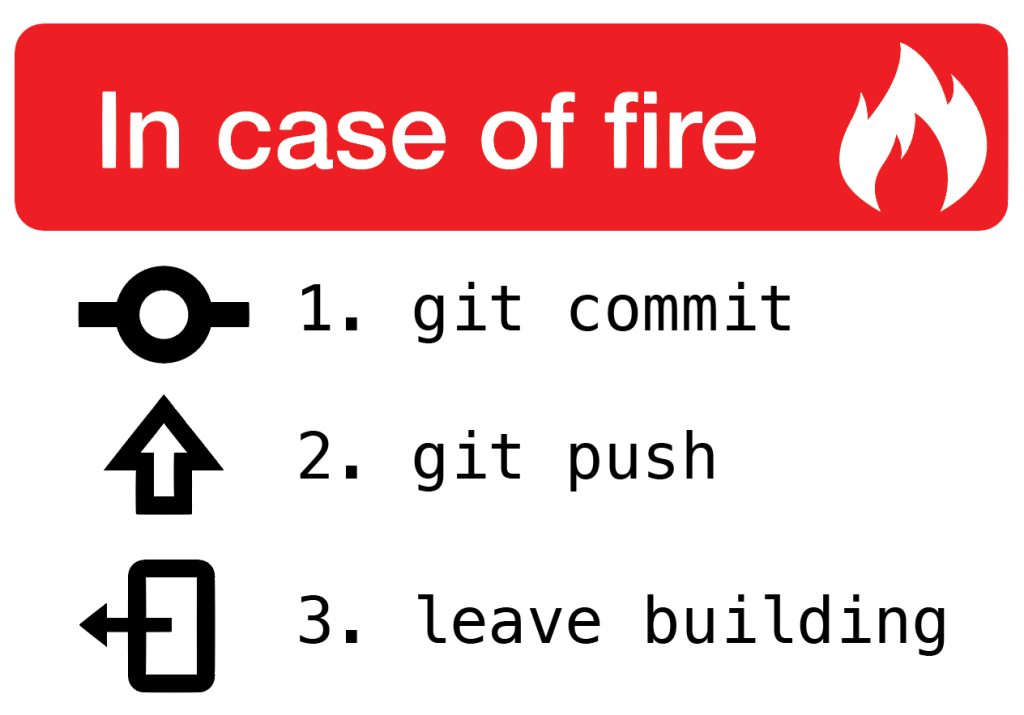
\includegraphics[scale=0.5]{images/incaseoffire.png}};
  \end{tikzpicture}
\end{frame}

\begin{frame}{Trabajar con Remotos - Seguimiento}
  \begin{itemize}
    \item \alert{Crear una rama de seguimiento}
      \mint{console}| $ git checkout --track <remoto>/<rama>|
      {\scriptsize La rama se llamará \texttt{<rama>} y nos moveremos a ella}
      \mint{console}| $ git checkout -b <rama> <remoto>/<rama>|
    \item \alert{Asignar seguimiento a una rama creada}
      \mint{console}| $ git branch -u <remoto>/<rama>|
    \item \alert{Ver las ramas a la que hace seguimiento}
      \mint{console}| $ git branch -vv|
  \end{itemize}
  Cuando hacemos \texttt{clone}, automáticamente \texttt{master} hace seguimiento de \texttt{origin/master}
\end{frame}


%  Guardado rápido
\begin{frame}{Guardado rápido}
  \begin{columns}[onlytextwidth]
    \column{0.3\textwidth}
    
\includegraphics[scale=0.9]{images/gitstash}
    \column{0.7\textwidth}
    \begin{itemize}
      \item \alert{Guardar los cambios}
        \mint{console}| $ git stash|
        \mint{console}| $ git stash save 'mensaje'|
      \item \alert{Guardar sólo los cambios preparados}
          \mint{console}| $ git stash --keep-index|
      \item \alert{Guardar de archivos no rastreados}
          \mint{console}| $ git stash -u|
      \item \alert{Guardar de forma selectiva}
          \mint{console}| $ git stash --patch|
    \end{itemize}
  \end{columns}
\end{frame}

\begin{frame}{Guardado rápido}
  \begin{columns}[onlytextwidth]
    \column{0.3\textwidth}
    
\includegraphics[scale=0.9]{images/gitstash}
    \column{0.7\textwidth}
    \begin{itemize}
      \item \alert{Listarlos}
          \mint{console}| $ git stash list|
      \item \alert{Aplicar un guardado}
          \mint{console}| $ git stash apply <stash@{x}>|
          {\scriptsize \ \ \texttt{--index}: recupera el estado}
      \item \alert{Aplicar y sacar un guardado}
          \mint{console}| $ git stash pop <stash@{x}>|
      \item \alert{Crear una rama}
          \mint{console}| $ git stash branch <rama> <stash@{x}>|
    \end{itemize}
    {\scriptsize Si no se especifica \texttt{<stash@{x}>}, Git selecciona el más reciente.}
  \end{columns}
\end{frame}

\begin{frame}{Guardado rápido}
  \begin{columns}[onlytextwidth]
    \column{0.3\textwidth}
    
\includegraphics[scale=0.9]{images/gitstash}
    \column{0.7\textwidth}
    \begin{itemize}
      \item \alert{Mostrar las diferencias}
          \mint{console}| $ git stash show <stash@{x}>|
      \item \alert{Limpiar el stash} \warnning
          \mint{console}| $ git stash clear|
      \item \alert{Sacar un guardado} \warnning
          \mint{console}| $ git stash drop <stash@{x}>|
    \end{itemize}
  \end{columns}
\end{frame}


%  Etiquetas
\begin{frame}[fragile]{Etiquetado - Creación y eliminación}
  \begin{columns}[T,onlytextwidth]
    \column{0.6\textwidth}
    \begin{itemize}
      \item
      \only<1>{
        \alert{Etiquetas Ligeras} \\
        Puntero a commit
        \mint{console}|  $ git tag <nombre-tag>|}
      \only<2>{
        \alert{Etiquetado tardío} \\
        \mint{console}|  $ git tag -a <nombre-tag> <SHA-1>|}
      \item
      \only<1>{
        \alert{Etiquetas Anotadas} \\
        Puntero, mensaje, etiquetador...
        \mint{console}|  $ git tag -a <nombre-tag> -m 'msj'|}
      \only<2>{
        \alert{Eliminar etiqueta} \warnning \\
        \mint{console}|  $ git tag -d <nombre-tag>|}
    \end{itemize}
    \column{0.4\textwidth}
      \begin{tikzpicture}
  \gitDAG[grow up sep = 1.5em]{
    H -- I -- J -- K -- L
  };
  % Tag reference
  \gittag
    [v0p9]       % node name
    {v0.9}       % node text
    {left=of H} % node placement
    {H}          % target
  \gittag
    [v1p0]       % node name
    {v1.0}       % node text
    {left=of L} % node placement
    {L}          % target
  % Remote branch
  \gitremotebranch
    [origmaster]    % node name
    {\tiny origin/master} % node text
    {right=of J}    % node placement
    {J}             % target
  % Branch
  \gitbranch
    {master}      % node name and text
    {right=of L} % node placement
    {L}          % target
  % HDAD reference
  \gitHEAD
    {right=of master} % node placement
    {master}          % target
\end{tikzpicture}

  \end{columns}
\end{frame}

\begin{frame}[fragile]{Etiquetado - Listado}
  \begin{columns}[T,onlytextwidth]
    \column{0.6\textwidth}
    \begin{itemize}
      \item \alert{Todas}
        \mint{console}|  $ git tag|
      \item \alert{Por patrón}
        \mint{console}|  $ git tag -l 'v1*'|
      \item \alert{Específica}
        \mint{console}|  $ git show <nombre-tag>|
    \end{itemize}
    \column{0.4\textwidth}
      \begin{tikzpicture}
  \gitDAG[grow up sep = 1.5em]{
    H -- I -- J -- K -- L
  };
  % Tag reference
  \gittag
    [v0p9]       % node name
    {v0.9}       % node text
    {left=of H} % node placement
    {H}          % target
  \gittag
    [v1p0]       % node name
    {v1.0}       % node text
    {left=of L} % node placement
    {L}          % target
  % Remote branch
  \gitremotebranch
    [origmaster]    % node name
    {\tiny origin/master} % node text
    {right=of J}    % node placement
    {J}             % target
  % Branch
  \gitbranch
    {master}      % node name and text
    {right=of L} % node placement
    {L}          % target
  % HDAD reference
  \gitHEAD
    {right=of master} % node placement
    {master}          % target
\end{tikzpicture}

  \end{columns}
\end{frame}

\begin{frame}[fragile]{Etiquetado - Compartir}
  \begin{columns}[T,onlytextwidth]
    \column{0.6\textwidth}
    \texttt{git push} no transfiere etiquetas a remotos
    \begin{itemize}
      \item \alert{Todas}
        \mint{console}|  $ git push origin --tags|
      \item \alert{Específica}
        \mint{console}|  $ git push origin <nombre-tag>|
    \end{itemize}
    \column{0.4\textwidth}
      \begin{tikzpicture}
  \gitDAG[grow up sep = 1.5em]{
    H -- I -- J -- K -- L
  };
  % Tag reference
  \gittag
    [v0p9]       % node name
    {v0.9}       % node text
    {left=of H} % node placement
    {H}          % target
  \gittag
    [v1p0]       % node name
    {v1.0}       % node text
    {left=of L} % node placement
    {L}          % target
  % Remote branch
  \gitremotebranch
    [origmaster]    % node name
    {\tiny origin/master} % node text
    {right=of J}    % node placement
    {J}             % target
  % Branch
  \gitbranch
    {master}      % node name and text
    {right=of L} % node placement
    {L}          % target
  % HDAD reference
  \gitHEAD
    {right=of master} % node placement
    {master}          % target
\end{tikzpicture}

  \end{columns}
\end{frame}

\begin{frame}[fragile]{Etiquetado - Sacar una etiqueta}
  \begin{columns}[T,onlytextwidth]
    \column{0.6\textwidth}
    Para colocar en el directorio de trabajo una versión, es necesario crear una nueva rama en esa etiqueta.
    \mint{console}|  $ git checkout -b <n-rama> <n-tag>|
    \uncover<2>{
    \vspace{0.5cm}
    Ejemplo:
    \mint{console}|  $ git checkout -b version0p9 v0.9|
    }
    \column{0.4\textwidth}
      \only<1>{\begin{tikzpicture}
  \gitDAG[grow up sep = 1.5em]{
    H -- I -- J -- K -- L
  };
  % Tag reference
  \gittag
    [v0p9]       % node name
    {v0.9}       % node text
    {left=of H} % node placement
    {H}          % target
  \gittag
    [v1p0]       % node name
    {v1.0}       % node text
    {left=of L} % node placement
    {L}          % target
  % Remote branch
  \gitremotebranch
    [origmaster]    % node name
    {\tiny origin/master} % node text
    {right=of J}    % node placement
    {J}             % target
  % Branch
  \gitbranch
    {master}      % node name and text
    {right=of L} % node placement
    {L}          % target
  % HDAD reference
  \gitHEAD
    {right=of master} % node placement
    {master}          % target
\end{tikzpicture}
}
      \only<2>{\begin{tikzpicture}
  \gitDAG[grow up sep = 1.5em]{
    H -- I -- J -- K -- L
  };
  % Tag reference
  \gittag
    [v0p9]       % node name
    {v0.9}       % node text
    {left=of H} % node placement
    {H}          % target
  \gittag
    [v1p0]       % node name
    {v1.0}       % node text
    {left=of L} % node placement
    {L}          % target
  % Remote branch
  \gitremotebranch
    [origmaster]    % node name
    {\tiny origin/master} % node text
    {right=of J}    % node placement
    {J}             % target
  % Branch
  \gitbranch
    {master}      % node name and text
    {right=of L} % node placement
    {L}          % target
  \gitbranch
    {version0p9}      % node name and text
    {right=of H}% node placement
    {H}          % target
  % HDAD reference
  \gitHEAD
    {above=of version0p9} % node placement
    {version0p9}          % target
\end{tikzpicture}
}
  \end{columns}
\end{frame}


%  gitignore
\begin{frame}[fragile]{.gitignore}
  \begin{columns}[onlytextwidth]
    \column{0.35\textwidth}
    \begin{itemize}
      \item \alert{Comentarios} \mint[style=bw]{bash}|#|
      \item \alert{Patrones glob} \mint[style=bw]{bash}|*, [abc], ?, [0-9]|
      \item \alert{Directorios} \mint[style=bw]{bash}|/|
      \item \alert{Negación} \mint[style=bw]{bash}|!|
    \end{itemize}
    \column{0.65\textwidth}
    \begin{exampleblock}{Ejemplo de .gitignore}
    \begin{minted}[bgcolor=solarized-base1!12, autogobble=true, fontsize=\scriptsize]{bash}
      # ignora todos los archivos terminados en .a y .o
      *.[ao]
      # pero no lib.a
      !lib.a
      # ignora el archivo sum.cpp del directorio
      /sum.cpp
      # ignora todos los archivos del directorio build/
      build/
      # ignora los .txt del directorio doc/
      doc/*.txt
      # ignora los .txt de doc/ y sus subdirectorios
      doc/**/*.txt
      claves_secretas # ESTE NO LO IGNORA PORQUE EL COMENTARIO ESTÁ EN LA MISMA LÍNEA
    \end{minted}
  \end{exampleblock}
  \end{columns}
\end{frame}


%  Configuración
\begin{frame}[fragile]{Configuración en Git - Niveles de configuración}
  \begin{center}
  \begin{tikzpicture}[
    scale=0.95,
    start chain=1 going below,
    start chain=2 going left,
    node distance=1mm,
    desc/.style={
      scale=0.95,
      on chain=2,
      rectangle,
      rounded corners,
      draw=solarized-base01,
      semithick,
      text centered,
      text width=3cm,
      minimum height=1.2cm,
      fill=solarized-green!30
      },
    level/.style={
      scale=0.95,
      on chain=1,
      minimum height=12mm,
      text width=7.5cm
    },
    every node/.style={font=\sffamily}
  ]
  % Levels
  \node [level] (Nivel 3) {\alert{.git/config} \\
  Específico para cada repositorio};
  \node [level] (Nivel 2) {\alert{$\sim$/.gitconfig}  o \alert{$\sim$/.config/git/config} \\
  Específico para cada usuario};
  \node [level] (Nivel 1) {\alert{/etc/config} \\
  Común a todos los usuarios y repositorios};
  % Descriptions
  \chainin (Nivel 3);
  \node [desc] (--local) {\texttt{$--$local}};
  \node [desc, continue chain=going below] (--global) {\texttt{$--$global}};
  \node [desc] (--system) {\texttt{$--$system}};
  \end{tikzpicture}
  \vspace{0.5cm}
  \begin{minted}{console}
                 $ git config --global <opciones>
  \end{minted}
  \end{center}
\end{frame}

\begin{frame}[fragile]{Configuración en Git - Algunos comandos}
  \alert{Identidad}
  \begin{minted}{console}
    $ git config --global user.name "Nombre Apellido Apellido"
    $ git config --global user.email email@email.com
  \end{minted}
  \alert{Editor}
  \begin{minted}{console}
    $ git config --global user.editor gedit
  \end{minted}
  \alert{Colores}
  \begin{minted}{console}
    $ git config --global color.ui true
  \end{minted}
\end{frame}

\begin{frame}[fragile]{Configuración en Git - Algunos comandos}
  \alert{Mensaje para commit por defecto}
  \begin{minted}{console}
    $ git config --global commit.template path/.gitmessage.txt
  \end{minted}
  \alert{Gitignore global}
  \begin{minted}{console}
    $ git config --global core.excludesfile path/.gitignore_global
  \end{minted}
  \alert{Ver la configuración actual}
  \begin{minted}{console}
    $ git config --global --list
  \end{minted}
\end{frame}

\begin{frame}[fragile]{Configuración en Git - Alias de Git}
  \alert{¡Nuestros propios comandos!}
  \begin{minted}{console}
    $ git config --global alias.<mi-alias> 'comando'
  \end{minted}
  Algunos ejemplos:
  \begin{minted}{console}
    $ git config --global alias.co checkout
    $ git config --global alias.br branch
    $ git config --global alias.ci commit
    $ git config --global alias.st status
  \end{minted}
  \begin{minted}{console}
    $ git config --global alias.unstage 'reset HEAD --'
    $ git config --global alias.last 'log -1 HEAD'
  \end{minted}

\end{frame}


%  Utilización de SSH en GitHub
\begin{frame}{Utilización de la clave pública SSH en \faGithub\ GitHub}
  Las claves SSH se almacenan en \texttt{$\sim$/.ssh}
  \begin{itemize}
    \item \alert{Generación}
    \mint{console}| $ ssh-keygen|
    \item \alert{Configuración} \\
    Id a \texttt{configuración} en Github y añadir la clave contenida en \texttt{$\sim$/.ssh/id\_rsa.pub} \\
    \warnning \ {\color{solarized-red}No compartas el privado}
    \item \alert{Clonación por SSH}
    \mint{console}| $ git clone git@github.com:user/repo.git|
  \end{itemize}

  \begin{tikzpicture}[remember picture,overlay]
    \node[anchor=north east,inner ysep=40pt, inner xsep=20pt] at (current page.north east) {
\includegraphics[scale=0.15]{images/logoGithub.png}};
  \end{tikzpicture}

\end{frame}


% TODO Montar un servidor (Gitlab)
% \input{sections/gitlab}

% TODO githubEducation
% \begin{frame}{GitHub Education}
  \begin{center}
  \begin{figure}
    
\includegraphics[scale=0.2]{images/githubEducation}
  \end{figure}
  \href{https://education.github.com}{\Large{education.github.com}}
  \end{center}

\end{frame}


\begin{frame}[standout]
  \whiteTitle
  \maketitle
  \begin{tikzpicture}[remember picture,overlay]
    \node[anchor=north east,inner sep=40pt] at (current page.north east) {
\includegraphics[scale=0.27]{images/logoGitw.png}};
    \node[anchor=south east,inner sep=40pt] at (current page.south east) {
\includegraphics[scale=0.3]{images/logoUCAw.png}};
  \end{tikzpicture}
\end{frame}

\end{document}
